In our model, the population of consumers can either feed on an abiotic resource following a chemostat-like dynamics (Equation \ref{eq:chemostat_resource_dynamics}) or on a biotic resource following a logistic-like dynamics (Equation \ref{eq:logistic_resource_dynamics}). The chemostat model depends on the resource inflow rate $a$ and the outflow rate $b$ while the logistic model depends on the resource intrinsic growth rate $r$ and the carrying capacity $K$. To make the outcome of the two models comparable, we recommend using parameter values that make the two model equivalent in achieved equilibrium consumer population size. Here we derive the correspondence between the parameters of the two models. Details are provided in the \textit{Mathematica} notebook accompanying this appendix.\\

Consider a population of asexual consumers having access to a single resource in a single habitat-patch. For simplicity, we assume a monomorphic population with respect to the ecological trait $x$ such that every individual has an optimal attack rate $1$ on the resource. This is equivalent to assuming that individuals have various ecological trait values but that the selection coefficient $s$ is zero. Because we are concerned with the ecological dynamics, we assume that the population does not evolve. The dynamics of the resources, assuming they are fast and they reach equilibrium before the population size changes, are

\begin{equation}
    \frac{dR}{dt} = a - (b + N)\,R
\end{equation}

for the chemostat model, where $N$ is the population size and $R$ is the concentration of the resource at a given point in time. This gives the equilibrium resource concentration

\begin{equation}
    R^* = \frac{a}{b+N}
\end{equation}

For the logistic model, the dynamics are

\begin{equation}
    \frac{dR}{dt} = r\,\bigg(1-\frac{R}{K}\bigg)\,R-N\,R
\end{equation}

which gives the equilibrium resource concentration

\begin{equation}
    R^* = \frac{K\,(r-N)}{r}
\end{equation}

We assume that the discrete-time dynamics of the consumer population are described by

\begin{equation}
    N_{t+1} = (1 - d + R^*)\,N_t
    \label{eq:recursion}
\end{equation}

where $d$ is the per capita death rate and $R^*$ represents the reproductive success of individuals according to Equation \ref{eq:fitness}. The sensitivity of the consumer population growth on the parameters of the underlying resource dynamics are shown in Figure \ref{fig:effect_of_resource_dynamics_on_population_dynamics}. At ecological equilibrium $N_{t+1} = N_t = N^*$, which we can solve for the chemostat model:

\begin{figure}
    \centering
    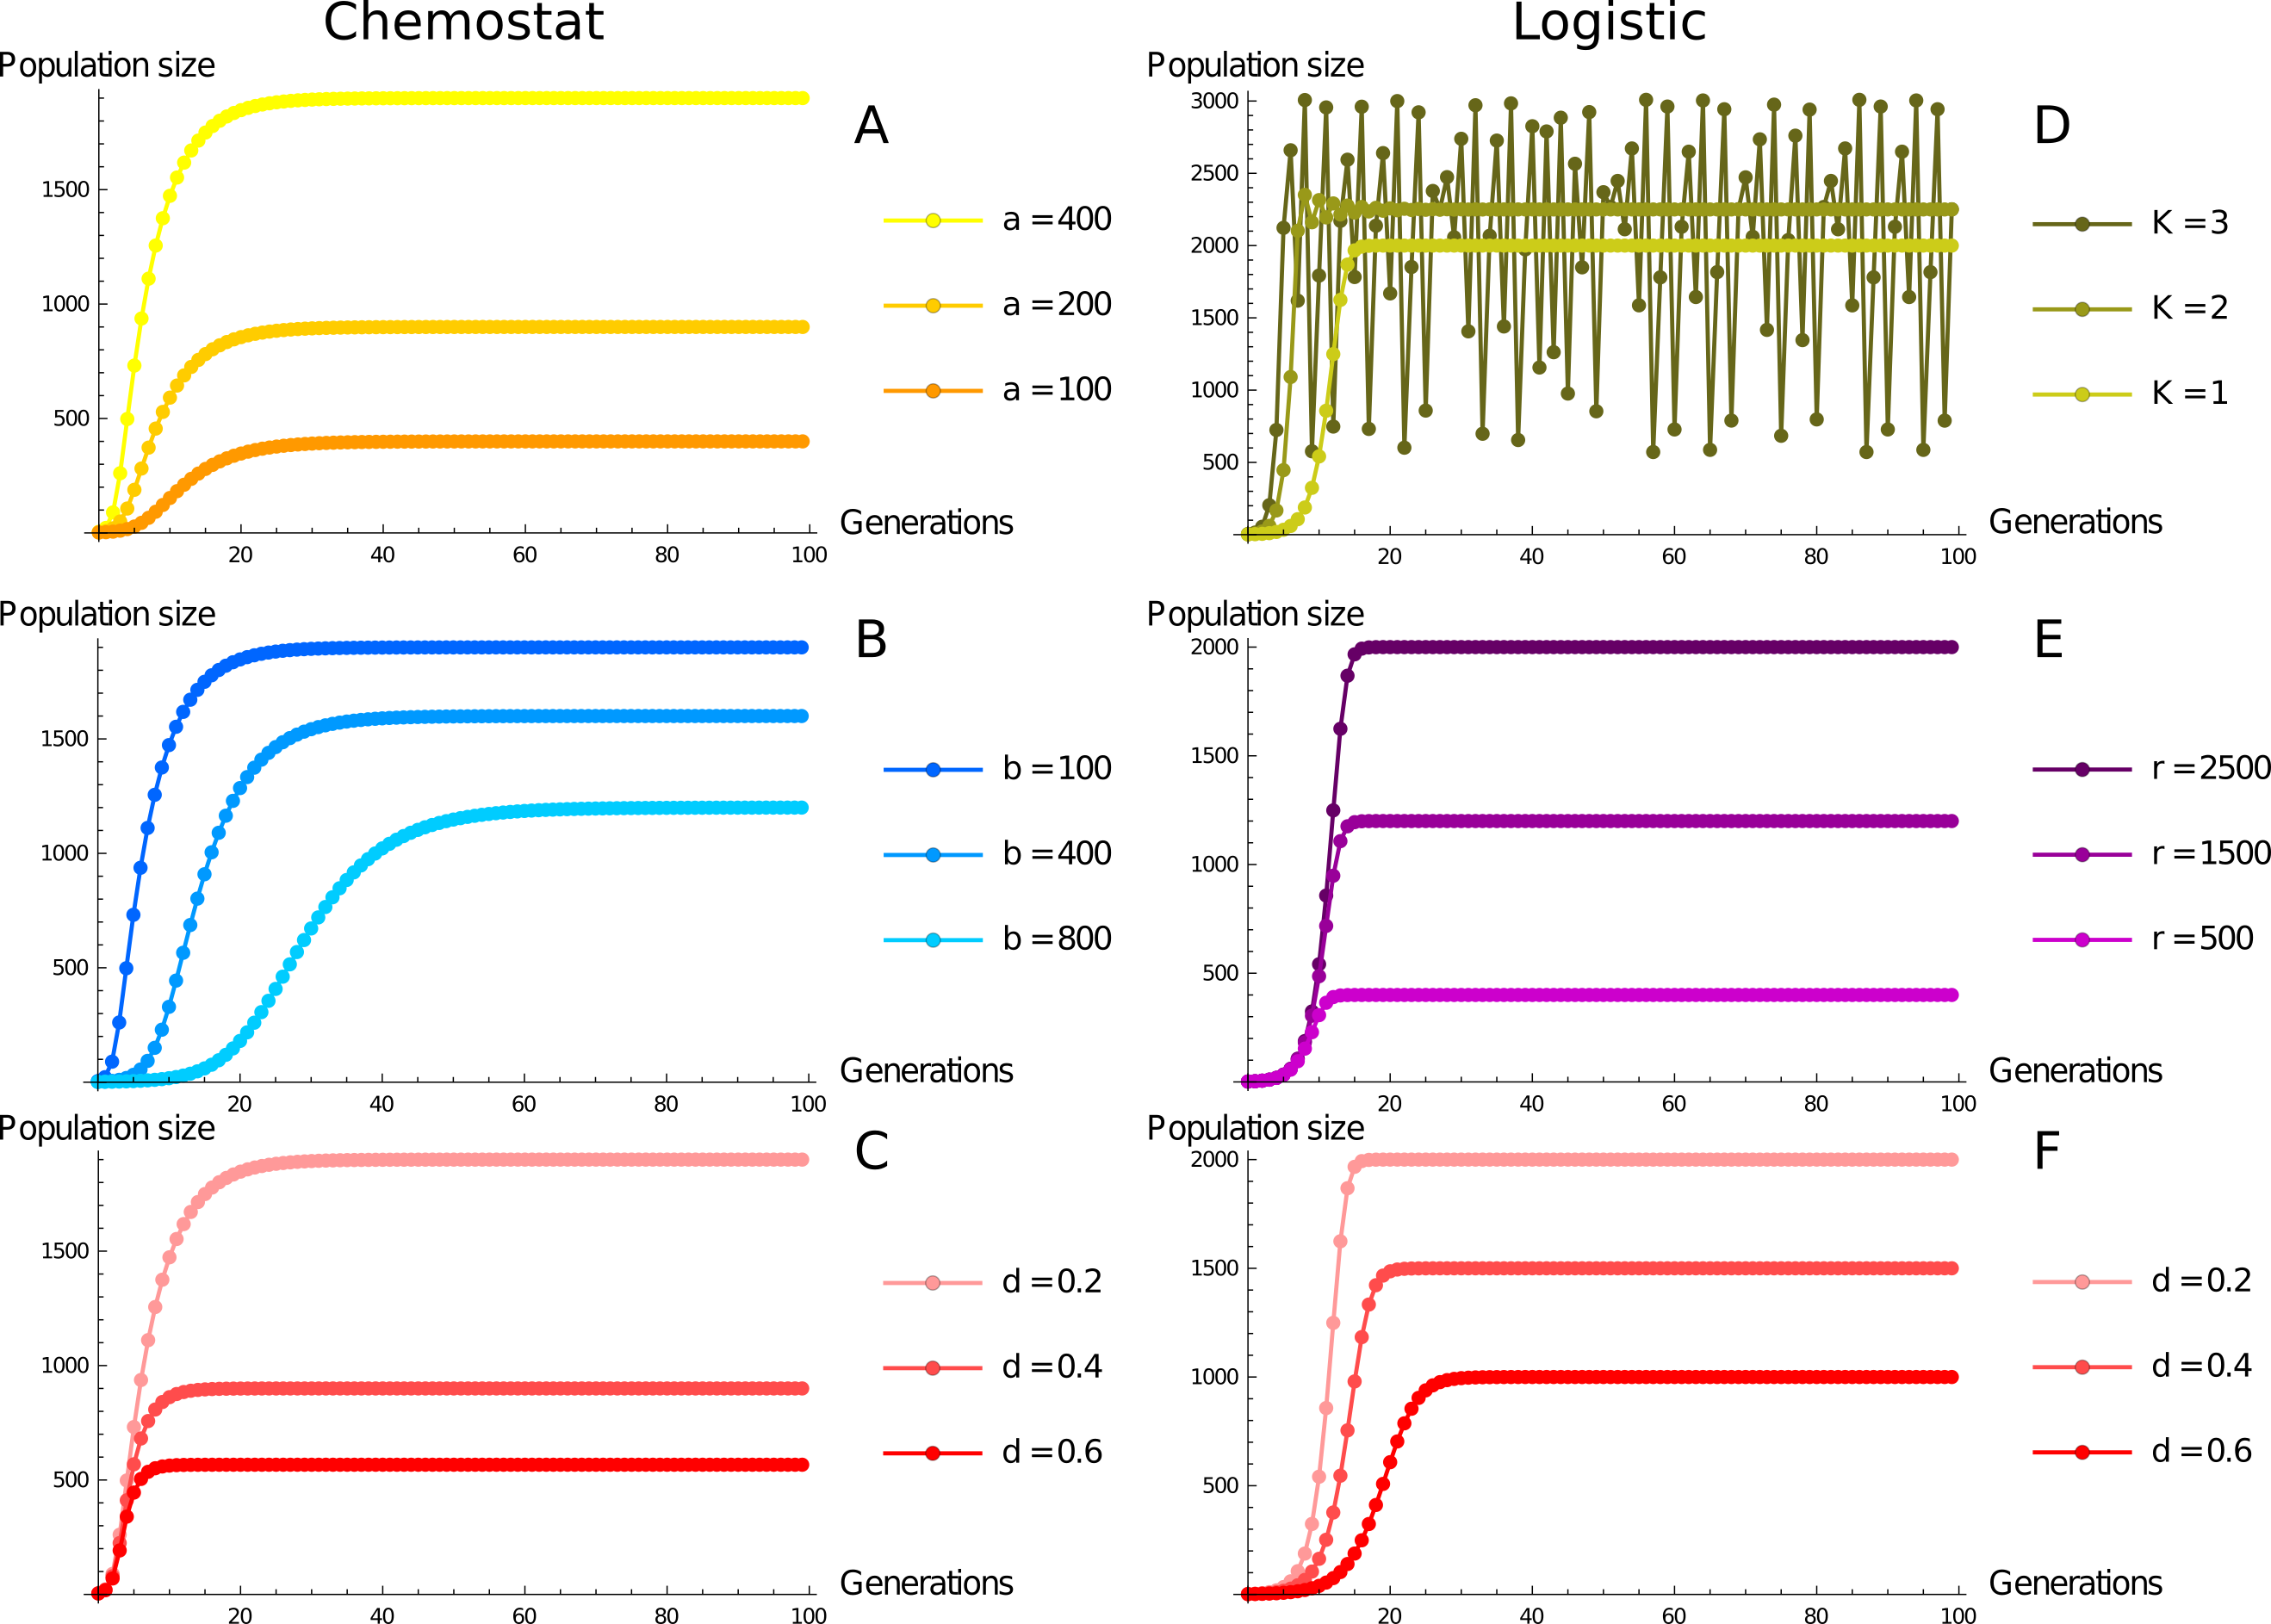
\includegraphics[width=\textwidth]{figures/population_dynamics_with_different_resource_dynamics.png}
    \caption{The effect of resource dynamics parameters on the dynamics of the consumer population. (A--C) Chemostat resource dynamics. (D--F) Logistic resource dynamics. (A) Effect of the resource inflow rate $a$. (B) Effect of the resource outflow rate $b$. (C) Effect of the death rate $d$ in a chemostat model. (D) Effect of the resource carrying capacity $K$. Note that higher values can produce chaotic consumer population dynamics. (E) Effect of the intrinsic growth rate of the resource $r$. (F) Effect of the death rate $d$ in a logistic model. Only one parameter was varied at a time. Fixed parameter values: $a = 400$, $b = 100$, $K = 1$, $r = 2500$, $d = 0.2$.}
    \label{fig:effect_of_resource_dynamics_on_population_dynamics}
\end{figure}

\begin{equation}
    N^* = \frac{a}{d}-b
\end{equation}

and for the logistic model:

\begin{equation}
    N^* = r\,\bigg(1-\frac{d}{K}\bigg)
\end{equation}

Therefore, parameter values of the chemostat and the logistic model such that both models yield the same equilibrium population size must satisfy the equality:

\begin{equation}
    \frac{a}{d}-b = r\,\bigg(1-\frac{d}{K}\bigg)
\end{equation}

Figure \ref{fig:chemostat_vs_logistic} shows two equivalent simulations of the deterministic population dynamics (Equation \ref{eq:recursion}) under the two resource dynamical models, with parameter values shown in Table \ref{tab:parameters}.

\begin{figure}
    \centering
    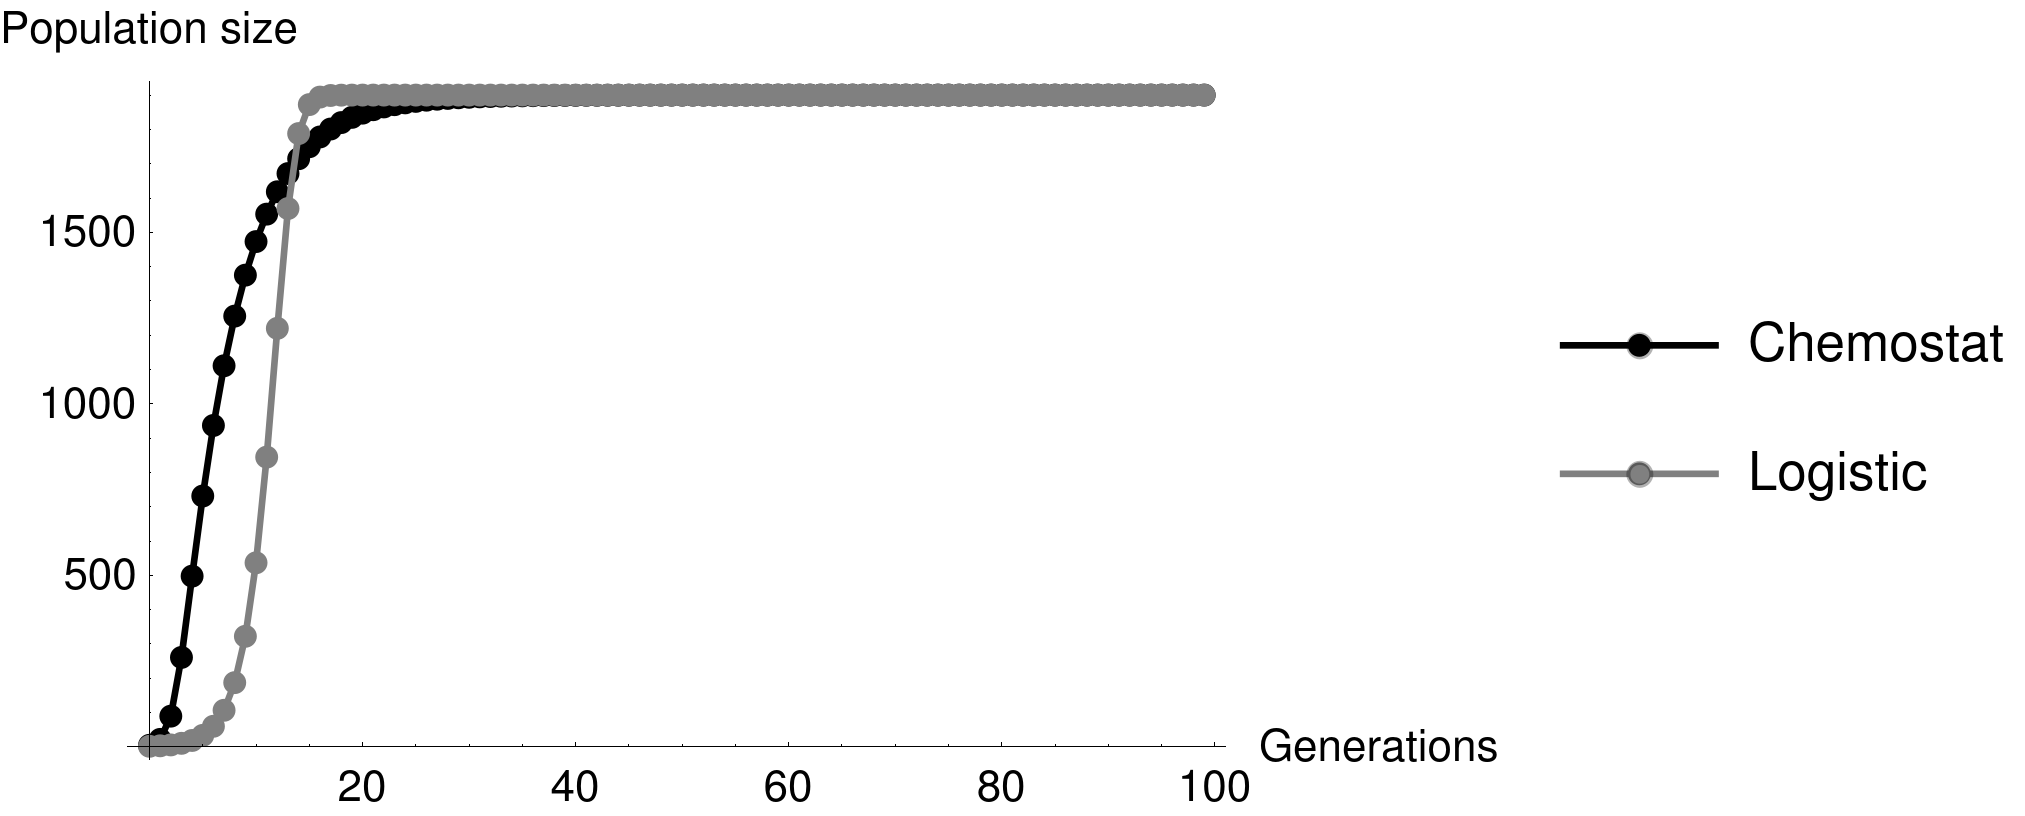
\includegraphics[width=0.9\textwidth]{figures/chemostat_vs_logistic.png}
    \caption{Population growth under two models of resource dynamics: a chemostat model representing an abiotic resource flowing through the landscape, and a logistic model representing a biotic resource with its own intrinsic growth. Both simulations were parametrized so as to reach the same equilibrium population size of 1900 individuals. Parameters: $a = 400$, $b = 100$, $K = 1$, $r = 2375$, $d = 0.2$.}
    \label{fig:chemostat_vs_logistic}
\end{figure}
